\section[BiCG]{BiCG}
{\bf Gegeben: }
\begin{quote}
$Ax=b$, $A \in \cnn$, $A$ regul�r.
\end{quote}
{\bf Gesucht: }
\begin{quote}
$r^m\in K_m(A,r^0)$, s.d.
\begin{equation} \label{petgalbed}
r^m \perp K_m(A^H,\tilde r^0).
\end{equation}
\end{quote}
\eqref{petgalbed} hei"st \textsl{Petrov-Galerkin}-Bedingung. \\
Erinnerung an unsymmetrischen Lanczos:
\begin{equation} \label{unsymm_lanc}
\left\{ \quad
\begin{array}{rcl}
AV_m &=& V_{m+1}T_{m+1,m} \\ A^HW_m &=& W_{m+1}\overline{T}_{m+1,m}
\end{array} \right.
\end{equation}
mit
\begin{eqnarray*}
 T_{m+1,m}=
 \left(\begin{array}{cccc}
                        \alpha_1  & \delta_2  & & \\
                        \delta_2  & \alpha_2 & \ddots  & \\
                                  & \ddots   & \ddots  & \delta_m \\
                                  &          & \ddots  & \alpha_{m} \\
					    &          &         & \delta_{m+1}
               \end{array}\right)
\end{eqnarray*}
mit $\alpha_i=\langle Av^i,w^i\rangle$ und $\delta_i^2=\langle \tilde v_i,\tilde w_i\rangle$ aus Algorithmus~\ref{unsymmetrisches Lanczos-Verfahren}.
Setze
\begin{eqnarray*}
 T_m=
 \left(\begin{array}{cccc}
                        \alpha_1  & {\delta}_2  & & \\
                        {\delta}_2  & \alpha_2 & \ddots  & \\
                                  & \ddots   & \ddots  & {\delta}_m \\
                                  &          & {\delta}_m  & \alpha_m
               \end{array}\right) \in \cmm.
\end{eqnarray*}
\begin{lem}
Sei $x^m=x^0+V_mz^m$, $r^m=b-Ax^m$. Dann erf"ullt $r^m$ die Bedingung \eqref{petgalbed} genau dann, wenn
\begin{equation} \label{eigT}
T_mz^m=\delta_1e^1
\end{equation}
gilt.
\end{lem}
\begin{proof}
$r^m = r^0-AV_mz^m$
\begin{eqnarray*} \begin{array}{rcl}
r^m \perp K_m(A,\tilde r^0) & \Leftrightarrow & \langle r^m,W_my \rangle = 0 \qquad \forall y \in \cn \\
& \Leftrightarrow & \langle r^0-AV_mz^m,W_my \rangle = 0 \\
& \Leftrightarrow & \langle r^0-V_{m+1}T_{m+1,m}z^m,W_my \rangle = 0 \\
& \Leftrightarrow & \langle V_{m+1}(\delta_1e^1-T_{m+1,m}z^m),W_my\rangle =0 \\
& \Leftrightarrow & \langle W_m^HV_{m+1}(\delta_1e^1-T_{m+1,m}z^m),y \rangle =0 \\
& \Leftrightarrow & W_m^HV_{m+1}(\delta_1e^1-T_{m+1,m}z^m)=0 \\
& \Leftrightarrow &  \left(\begin{array}{c|c} & 0 \\  \quad  \text{\Large $I_m$} \quad   & \vdots \\ & 0 \end{array}\right)\cdot (\delta_1e^1-T_{m+1,m}z^m)=0 \\
& \Leftrightarrow & \delta_1e^1-T_mz^m=0 \\
& \Leftrightarrow & T_mz^m = \delta_1e^1.\end{array} \end{eqnarray*} 
\end{proof}
\begin{bem}
Im allgemeinen Fall besitzt \eqref{eigT} nicht unbedingt eine L"osung, da $T_m$ singul"ar werden kann.
Ist aber $A=A^H$ hpd und $\tilde r^0=r^0$ im unsymmetrischen Lanczos, so wird der Prozess zum symmetrischen
Lanczos und $T_m=V_m^HAV_m$ hpd.
\end{bem}
\begin{defn}
Das KUV, welches Iterierte $x^m$ bestimmt mit \eqref{petgalbed}, hei"st \emph{BiCG-Verfahren}
(bi-konjugierte Gradienten). Im Spezialfall $A=A^H$ hpd, $\tilde r^0=r^0$ hei"st es CG-Verfahren.
\end{defn}

\begin{lem}
Sei $\xi \not = 0$ eine Nullstelle des BiCG-Polynoms, $r^m=p_m^{\text{BiCG}}(A)r^0$. 
Dann gilt: $\xi$ ist Eigenwert von $T_m$.
\end{lem}
\begin{proof}
Sei $p_m^{\text{BiCG}}(t)=(1-\frac{t}{\xi})q_{m-1}(t)$. Wegen \eqref{petgalbed} gilt
\begin{eqnarray*} \begin{array}{cl}
& \langle (I-\frac{1}{\xi}A)\underbrace{q_{m-1}(A)r^0}_{=V_mz^m},W_my\rangle =0 \qquad \forall y \in \cm \\
\Leftrightarrow & \langle (I-\frac{1}{\xi}A)V_mz^m,W_my\rangle =0 \\
\Leftrightarrow & \langle V_mz^m,W_my \rangle - \frac{1}{\xi}\langle AV_mz^m,W_my \rangle =0 \\
\Leftrightarrow & \langle z^m,y \rangle - \frac{1}{\xi}\langle V_{m+1}T_{m+1,m}z^m, W_my\rangle =0 \\
\Leftrightarrow & \langle z^m,y \rangle - \frac{1}{\xi}\langle T_mz^m,y\rangle =0 \\
\Leftrightarrow & z^m - \frac{1}{\xi}T_mz^m =0 \\
\Leftrightarrow & T_mz^m=\xi z^m.
\end{array} \end{eqnarray*} 
\end{proof}


Betrachte den Spezialfall $A=A^H$, $r^0=\tilde r^0$. Dann ist 
\begin{eqnarray*} \begin{array}{rcl}
T_m&=&V_m^HAV_m \quad \text{hermitesch}, \\
T_m&=&P^HD_mP, \quad P^HP=I, \quad D_m=\diag(d_1,\ldots,d_m).
\end{array} \end{eqnarray*} 
Andererseits
$$A=Q^H\Lambda Q, \quad Q^HQ=I,\quad \Lambda=\diag(\lambda_1,\ldots,\lambda_n).$$
Also
\begin{eqnarray*} \begin{array}{rcccl}
D_m&=&P^HT_mP&=&P^HV_m^HAV_mP \\
&&&=&P^HV_m^HQ^H\Lambda \underbrace{QV_mP}_{=:Y}.
\end{array} \end{eqnarray*}
Insbesondere gilt
\begin{eqnarray*}
d_i=\sum\limits_{j=1}^n\lambda_j |y_{ji}| \quad \text{mit } \sum|y_{ji}|^2=1.
\end{eqnarray*}
Die Eigenwerte von $T_m$ sind also gewichtete arithmetische Mittel der Eigenwerte von $A$, die sog. 
{\em Ritz-Werte}.
 
Wie bei CG kann man aus dem unsymmetrischen Lanzcos-Verfahren
eine Standardform des BiCG-Verfahrens herleiten. Wir geben hier lediglich das Resultat an:

\begin{alg}[BiCG, Fletcher 1973] \label{alg:bicg}
~               % um "Algorithmus" aus dem Kasten rauszubekommen
\vspace*{-2\baselineskip}       % um den Leeraum zu entfernen
\begin{algorithm}
  \begin{algorithmic}
    \STATE w\"ahle $x^0$, setze $r^0 = b-Ax^0$, w�hle $\tilde{r}^0,\ p^0=r^0,\ \tilde{p}^0=\tilde{r}^0$
    \FOR{$k = 0,1, \dots$ }
      \STATE $\gamma_k = \dfrac{\langle r^k, \tilde{r}^k \rangle}{\langle Ap^k, \tilde{p}^k \rangle}$
	\STATE $x^{k+1} = x^k + \gamma_k p^k$
	\STATE $r^{k+1} = r^k - \gamma_k Ap^k$
	\STATE $\rho_k= \dfrac{\langle r^{k+1},\tilde{r}^{k+1} \rangle}{\langle r^k, \tilde{r}^k \rangle}$
	\STATE $p^{k+1}=r^{k+1} + \rho_k p^k$
	\STATE $\tilde{r}^{k+1}=\tilde{r}^k - \overline{\gamma}_k A^H \tilde{p}^k$
	\STATE $\tilde{p}^{k+1}=\tilde{r}^{k+1} + \overline{\rho}_k \tilde{p}^k$
    \ENDFOR
  \end{algorithmic}
\end{algorithm}
\end{alg}

\begin{bem}
\begin{enumerate}
\item Man kann per vollst�ndiger Induktion aus Algorithmus~\ref{alg:bicg} direkt herleiten, dass f�r alle $k$ gilt
\[
r^k \perp K_k(A^H,\tilde{r}^0), \tilde{r}^k \perp K_k(A,r^0), Ap^k \perp \tilde{p}^i, A^H\tilde{p}^k \perp p^i, i=1,\ldots,k-1,
\]
und daraus dann, dass die Iterierten die Petrov-Galerkin Bedingung erf�llen.
\item 2 MVM pro Schritt ($Ap^k$ und $A^H \tilde{p}^k$)
\item Breakdowns: Lanczos Breakdown (erkennbar durch $\langle r^k, \tilde{r}^k \rangle=0$) und BiCG-Breakdown
			($T_k$ ist singul�r, d.h. es existiert keine Iterierte mit $r^k \bot K_k(A^H,\tilde{r}^0)$,
			erkennbar durch $\langle Ap^k, \tilde{p}^k \rangle =0$).
\end{enumerate}
\end{bem}

\begin{aufg}
F�hre BiCG f�r das Modellproblem III durch.
\end{aufg}

\begin{figure}[h!]
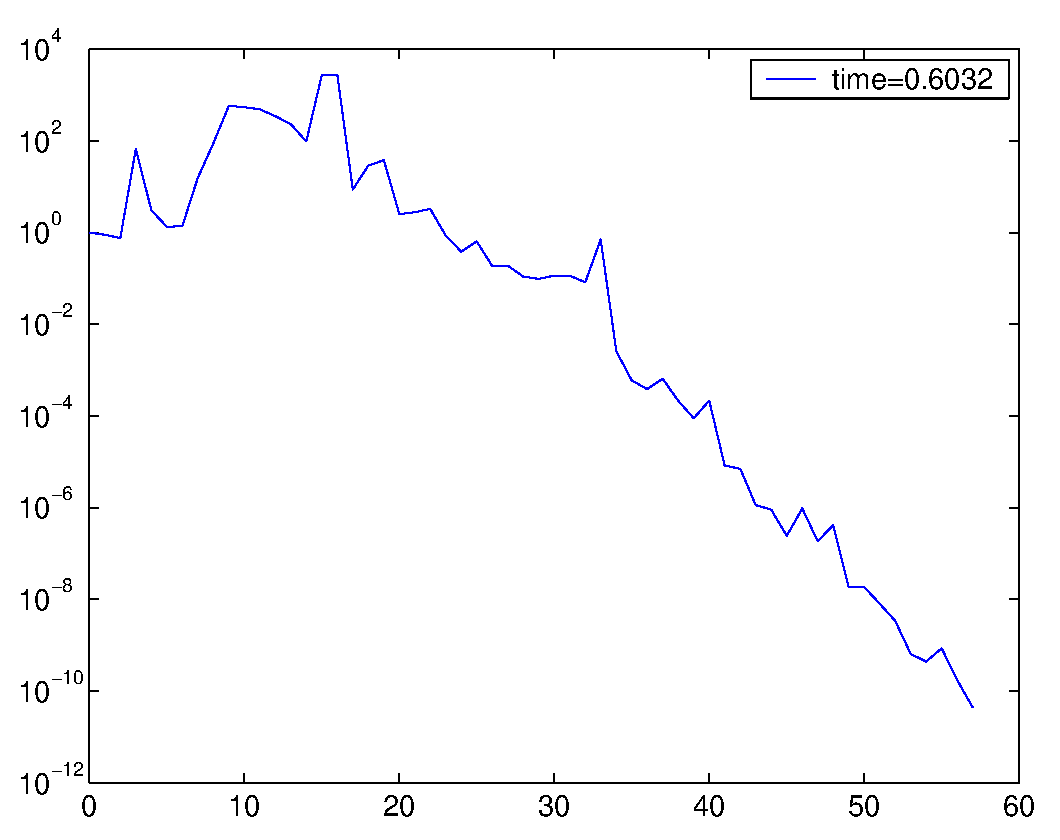
\includegraphics[scale=0.35]{eps/mp3bicgN20e50.eps}\hfill\includegraphics[scale=0.35]{eps/mp3bicgN20e1.eps}
\caption{Konvergenzgeschichte f"ur BiCG, Modellproblem III. Links:$N=20,
\epsilon = 50$, rechts $N=20, \epsilon = 1$}
\end{figure}


\begin{aufg}
Sei $A \neq A^H$, aber mit einer der folgenden speziellen Eigenschaften:
\begin{enumerate}
\item $A^H = \overline{A} \in \cnn$ (z.B. bei der Diskretisierung der Maxwell-Gleichungen in der Elektrodynamik)
\item $A^HJ = J^HA,\ J \in \cnn,\ J=J^H$ (man nennt $A$ dann auch {\em
$J$-hermitesch})
\item $A^TJ = J^TA,\ J \in \cnn$ (man nennt $A$ dann auch {\em $J$-symmetrisch})
\end{enumerate}
Zeige jeweils: F�r geeignete Wahl von $\tilde{r}^0$ (bzw. $w^0$) kann man den unsymmetrischen Lanczos-Prozess mit nur einer MVM mit $A$
(und eventuell einer zus�tzlichen mit $J$) durchf�hren
(dies �bertr�gt sich dann auch auf BiCG).
\end{aufg}